\documentclass[../master]{subfiles}
\begin{document}

\chapter{はじめに}
\section{宇宙での元素合成}
\label{seq::nucleaosynthesis}
身の回りには多種多様な物質が存在しており,
これらの物質は全て原子から構成されている.
現在の地球には水素(原子番号1)からウラン(原子番号92)までの元素が天然に存在してる.
原子は原子核と電子から構成されており,原子核は陽子と中性子で構成されることが知られている.
原子核に含まれる陽子の数が元素の原子番号となる.
現在までに天然と人工を合わせて118種類の元素が確認されている.
しかし,原始の宇宙では物質は存在せず,エネルギーで満たされていたと考えられている.
宇宙が膨張し温度が下がるにしたがって,陽子と中性子が生成され,
その後,原子核反応を起こすことで様々な原子核が合成された.
宇宙の初期には,水素とヘリウムと僅かな軽元素しか合成されなかった考えられている.
これは,質量数 ($A$) が5と8の原子核に安定な原子核が存在しないことに由来する.
初期の宇宙では陽子や中性子を捕獲して原子核が大きくなっていくが,
$A = $5と8の原子核が生成してもすぐに$A = $4 以下の軽い原子核に分裂してしまうのである.

%ヘリウムに比べて水素の方が多いため,水素を主成分とする恒星しか存在しなかったと考えられる.
宇宙に存在する元素のうち殆どが水素であるため,恒星は水素を主成分とする.
重力により収縮し中心温度が\SI{e7}{\kelvin}を超えると,
陽子(水素)同士が連鎖的に反応するようになる (ppチェイン).
ppチェインでは図\ref{fig::pp_chain}に示した3つの系列が重要とされる.
%chain~1 では3つの陽子から1つの${}^{3}\mathrm{He}$が形成され,
%2つ${}^{3}\mathrm{He}$から1つの$\alpha粒子と2つの陽子が生成される.
chain~1 では合計6つの陽子から1つの$\alpha$粒子と2つの陽子が生成される.
chain~2, 3 では合計で4つの陽子と1つの$\alpha$粒子から2つの$\alpha$粒子が生成される.
%chain~2, 3 では$A = $7
どの系列も最終的に4つの陽子から1つの${}^{4}\mathrm{He}$原子核($\alpha$粒子)が生成される.
ppチェインのように粒子(陽子や$3{}^{3}\mathrm{He}$など)が順番に一つずつ原子核に吸収される反応では,
$A = $8の壁を超えることはできない.
この壁を超えるためには$A = $4以下の原子核から$A = $9以上の原子核が直接生成されなければならない.
%\begin{gather}
%  {\rm p}({\rm p},\beta^{+}\nu){\rm d}({\rm p},\gamma){}^{3}{\rm He}({}^{3}{\rm He},2{\rm p})\alpha\label{eq::pp1}\\
%  {\rm p}({\rm p},\beta^{+}\nu){\rm d}({\rm p},\gamma){}^{3}{\rm He}(\alpha,\gamma){}^{7}{\rm Be}({\rm e}^{-},\nu){}^{7}{\rm Li}({\rm p},\alpha)\alpha\label{eq::pp2}\\
%  {\rm p}({\rm p},\beta^{+}\nu){\rm d}({\rm p},\gamma){}^{3}{\rm He}(\alpha,\gamma){}^{7}{\rm Be}({\rm p},\gamma){}^{8}{\rm B}(\beta^{+}\nu){}^{8}{\rm Be}(\alpha)\alpha\label{eq::pp3}
%\end{gather}
%\begin{gather}
%  \begin{array}{llll}
%    {\rm p} + {\rm p} \rightarrow & {\rm d} + \beta^{+} + \nu & &\\
%    & {\rm d} + {\rm p} \rightarrow & {}^{3}{\rm He} + \gamma &\\
%    & & {}^{3}{\rm He} + {}^{3}{\rm He} \rightarrow & {\rm \alpha} +2{\rm p}
%  \end{array}\label{eq::pp1}\\  
%  \begin{array}{llllll}
%    {\rm p} + {\rm p} \rightarrow & {\rm d} + \beta^{+} +\nu & & & &\\
%    & {\rm d} + {\rm p} \rightarrow & {}^{3}{\rm He} + \gamma & & &\\
%    & & {}^{3}{\rm He} + \alpha \rightarrow & {}^{7}{\rm Be} & &\\
%    & & & {}^{7}{\rm Be} + {\rm e}^{-} \rightarrow & {}^{8}{\rm Li} + \nu &\\
%    & & & & {}^{7}{\rm Li} + {\rm p} \rightarrow & \alpha + \alpha
%  \end{array}\label{eq::pp2}\\
%  \begin{array}{lllllll}
%    {\rm p} + {\rm p} \rightarrow & {\rm d} + \beta^{+} + \nu & & & & &\\
%    & {\rm d} + {\rm p} \rightarrow & {}^{3}{\rm He} + \gamma & & & &\\
%    & & {}^{3}{\rm He} + \alpha \rightarrow & {}^{7}{\rm Be} + \gamma & & &\\
%    & & & {}^{7}{\rm Be} + {\rm p} \rightarrow & {}^{8}{\rm B} + \gamma & &\\
%    & & & & {}^{8}{\rm B} \rightarrow & {}^{8}{\rm Be} + \beta^{+} + \nu &\\
%    & & & & & {}^{8}{\rm Be} \rightarrow & 3\alpha
%  \end{array}\label{eq::pp3}
%\end{gather}
\begin{figure}
  \centering
  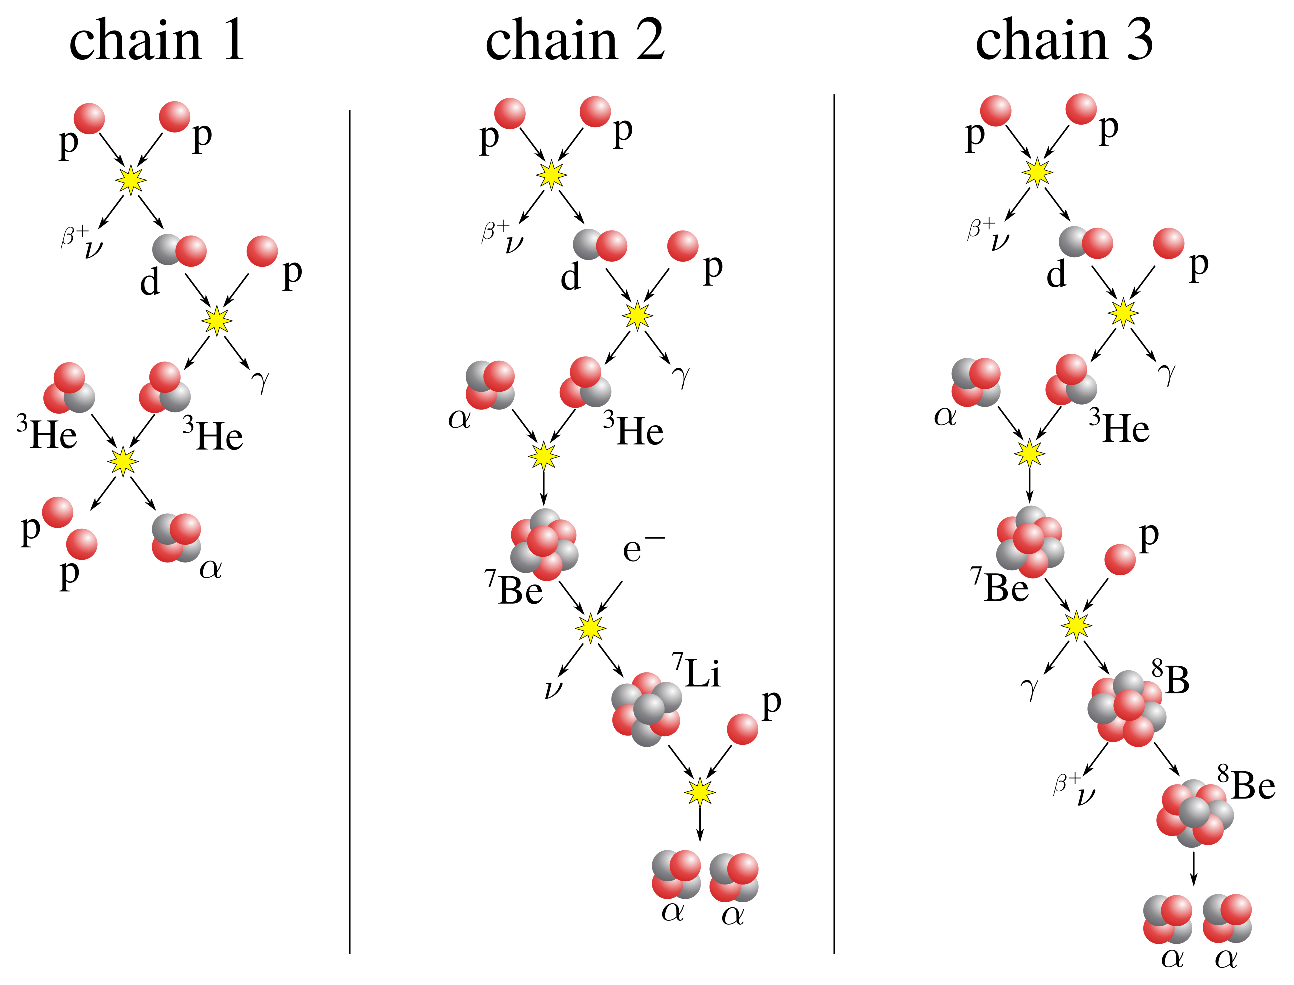
\includegraphics[clip, width=0.9\columnwidth]{pp_chain.eps}
  \caption{代表的なpp チェイン.pp チェインでは4つの陽子から1つの$\alpha$粒子が生成される.}
  \label{fig::pp_chain}
\end{figure}

ppチェインにより$\alpha$粒子が十分に生成された恒星では,
水素よりも重い$\alpha$粒子が恒星の中心に集まり$\mathrm{He}$コアを生成する.
$\mathrm{He}$コアが重力により圧縮され温度が約\SI{e8}{\kelvin}に達するとヘリウム燃焼が始まる.
$\mathrm{He}$コアには十分な量の$\alpha$粒子が存在するため,
図\ref{fig::triple_alpha}のように2つの$\alpha$粒子から2$\alpha$クラスター状態である${}^{8}\mathrm{Be}$が合成され,
さらに,${}^{8}\mathrm{Be}$が崩壊するより早くもう1つの$\alpha$粒子が
融合して${}^{12}\mathrm{C}$の励起状態 (${}^{12}\mathrm{C}^{*}$) が生成される反応が起こる.
このときに作られる${}^{12}\mathrm{C}^{*}$の多くはFred Hoyle が予言した$3\alpha$粒子の
共鳴状態 (Hoyle状態,$E_{x} = \SI{7.65}{\mega\electronvolt}$,$0_{2}^{+}$)~\cite{hoyle_state}となる.
このとき,${}^{12}{\rm C} (0_2^+)$が$\gamma$線を放出し脱励起すると${}^{12}\mathrm{C}$原子核が生成される
 (図\ref{fig::triple_alpha}~左) .
この3つの$\alpha$粒子から${}^{12}\mathrm{C}$が直接合成される反応はトリプルアルファ反応と呼ばれる.
トリプルアルファ反応が恒星中で起こることで$A = $4の$\alpha$粒子から
$A = $12の${}^{12}\mathrm{C}$が直接生成されるため,$A = $5, 8の壁を乗り越えることができ,
さらに重い$\mathrm{O}$や$\mathrm{Si}$などの合成へ進んでいく.
そのため,トリプルアルファ反応は宇宙元素合成において重要な原子核反応の1つである.
%\begin{equation}
%  \begin{array}{llll}
%%  \alpha(\alpha,\gamma){}^{8}{\rm Be}(\alpha,{}^{12}{\rm C}^{{\rm Hoyle}})
%%  \alpha(\alpha,\gamma){}^{8}{\rm Be}+\alpha\rightarrow{}^{12}{\rm C}^{{\rm Hoyle}}\label{eq::triplealpha}
%  %あとで矢印の絵を書こうかな
%    \alpha + \alpha \rightarrow & {}^{8}{\rm Be} & & \\
%    & {}^{8}{\rm Be} + \alpha \rightarrow & {}^{12}{\rm C}^{{\rm Hoyle}} &\\
%    & & {}^{12}{\rm C}^{{\rm Hoyle}} \rightarrow & {}^{12}{\rm C} + \gamma
%  \end{array}\label{eq::triplealpha}
%\end{equation}
\begin{figure}
  \centering
  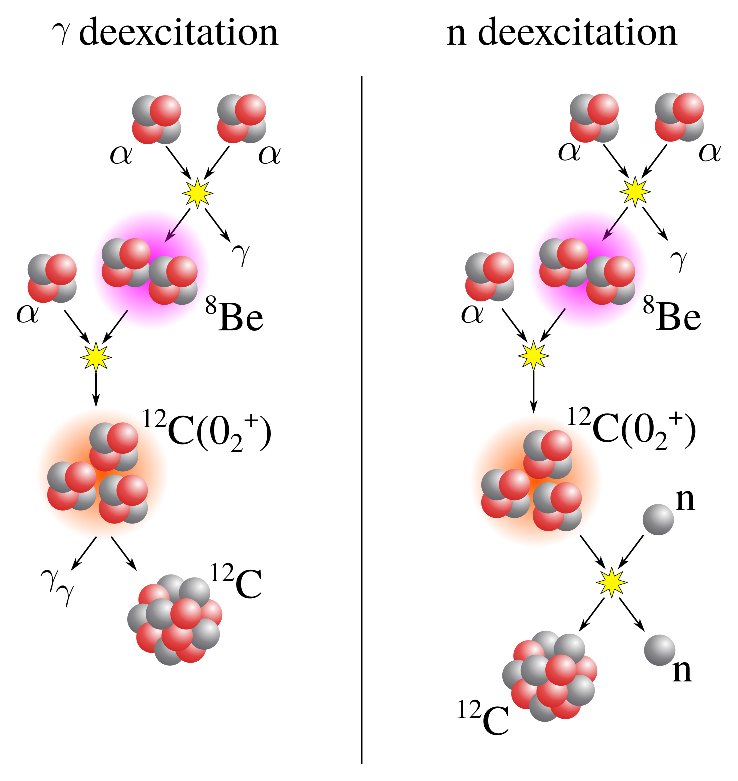
\includegraphics[clip, width=0.7\columnwidth]{triple_alpha.eps}
  %  \caption{トリプルアルファ反応.3つの$\alpha$粒子が反応し1つの${}^{12}{\rm C}$が生成される.}
  \caption[トリプルアルファ反応.]{トリプルアルファ反応.
    左は$\gamma$線を放出して脱励起するルート,右は中性子との非弾性散乱により脱励起するルートを表す.}
  \label{fig::triple_alpha}
\end{figure}

\section{高密度環境下でのトリプルアルファ反応}
\label{seq::triplealphareaction}
通常,トリプルアルファ反応で生成された$3\alpha$共鳴状態は図\ref{fig::triple_alpha} の左のように
$\gamma$線を放出することによって脱励起し,${}^{12}\mathrm{C}$の基底状態 (g.s.) になる.
近年,高密度環境下では$\gamma$線による脱励起以外に,
図\ref{fig::triple_alpha}~(右) のように粒子(陽子,中性子,$\alpha$粒子など)との
非弾性散乱による脱励起の反応率が増加することが指摘されている~\cite{hotdensemedium}.
これにより$0_2^+$状態からg.s.や$2_{1}^{+}\ (E_{x} = \SI{4.44}{\mega\electronvolt})$ への脱励起が増加し,
トリプルアルファ反応が劇的に促進されると考えられている.
粒子の中でも中性子は電荷を持っておらず,クーロン斥力を受けずに反応することができるため,
特にトリプルアルファ反応を促進する効果が大きい.

%\begin{equation}
%  \begin{array}{llll}
%    \alpha + \alpha \rightarrow & {}^{8}{\rm Be} & &\\
%    & {}^{8}{\rm Be} + \alpha \rightarrow & {}^{12}{\rm C}^{{\rm Hoyle}} &\\
%    & & {}^{12}{\rm C}^{{\rm Hoyle}} + {\rm X} \rightarrow & {}^{12}{\rm C} + {\rm X'}
%  \end{array}\label{eq::triplealpha_particle}
%\end{equation}

%\begin{figure}
%  \centering
%  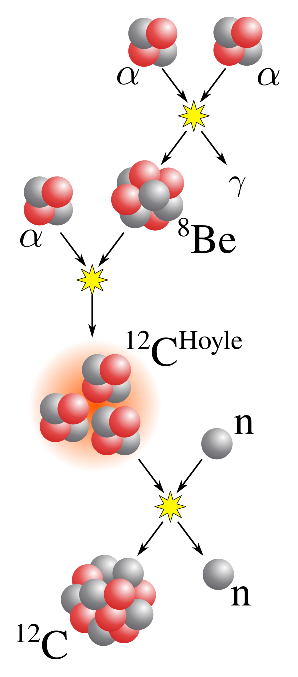
\includegraphics[clip, width=0.5\columnwidth]{triple_alpha_n.eps}
%  \caption[粒子との散乱により脱励起するトリプルアルファ反応.]{粒子との散乱により脱励起するトリプルアルファ反応.
%  この図では中性子と散乱する場合を表している.}
%  \label{fig::triple_alpha_n}
%\end{figure}%

%${}^{12}\mathrm{C}$と中性子の反応レートは
${}^{12}\mathrm{C}(0_2^+)(\mathrm{n}',\mathrm{n}){}^{12}\mathrm{C}$反応の
体積当たりの反応率は
\begin{equation}
  r = N_{\text{n}}N_{{}^{12}\mathrm{C}}\braket{\sigma v}% \si[per-mode=reciprocal]{\per\cubic\centi\metre\per\second}
  \label{eq::r}
\end{equation}
で与えられる.
ここで,$N_{\text{n}}$は中性子の個数密度,
$N_{{}^{12}\mathrm{C}}$は${}^{12}\mathrm{C}(0_2^+)$の個数密度を表す.
$\sigma$は中性子との散乱により始状態 ($0_2^+$) からg.s.または$2_{1}^{+}$状態へ脱励起する全断面積であり,
$v$は中性子と${}^{12}\mathrm{C}$の相対速度である.
相対速度がMaxwell分布に従うとすると,${}^{12}\mathrm{C}(0_2^+)(\mathrm{n'},\mathrm{n}){}^{12}\mathrm{C}$では,
\begin{equation}
  \braket{\sigma v}_{\mathrm{n'n}} =
  \left(\frac{8}{\pi\mu}\right)^{1/2}\left(\frac{1}{kT}\right)^{3/2}
  \int^{\infty}_{0}E'\sigma_{\mathrm{n'n}}(E')\exp(-E'/kT)dE'
  \label{eq::sigmann'}
\end{equation}
となる.
$T$は温度,$\mu$は換算質量,$\sigma_{\mathrm{n}'\mathrm{n}}$は${}^{12}\mathrm{C}(0_2^+)$の中性子非弾性散乱断面積である.
ここで上記の逆過程である ${}^{12}\mathrm{C}(\mathrm{n},\mathrm{n}'){}^{12}\mathrm{C}(0_2^+)$ を考えると,
\begin{equation}
  \braket{\sigma v}_{\mathrm{nn'}} = \left(\frac{2I'+1}{2I+1}\right)
  \exp(Q/kT)\braket{\sigma v}_{\mathrm{n'n}}
  \label{eq::sigman'n}
\end{equation}
という関係にある.
ここで,$I$および$I'$はそれぞれ始状態 (g.s.または$2_{1}^{+}$)および終状態 ($0_2^+$状態) のスピンである.
$Q$は\SI{-7.65}{\mega\electronvolt} (始状態がg.s.の場合) または
\SI{-3.21}{\mega\electronvolt} (始状態が$2_{1}^{+}$の場合) となる.
${}^{12}\mathrm{C} (0_2^+)$の中性子非弾性散乱による脱励起の寿命は
\begin{equation}
  \tau_{\mathrm{n'n}}\left[{}^{12}\mathrm{C} (0_2^+)\right] =
  (N_{\mathrm{n}}\braket{\sigma v}_{\mathrm{n'n}})^{-1} %\si{\second}
  \label{eq::tau}
\end{equation}
となる.

中性子非弾性散乱による脱励起の寿命と$\gamma$線による脱励起の寿命 ($\tau_{\gamma} = \SI{1.710e-13}{\second}$) との比を
$R$とすると,式\eqref{eq::sigmann'},\eqref{eq::sigman'n},\eqref{eq::tau}から
\begin{equation}
  R = 6.557\times10^{-6}\times\rho_{\mathrm{n}}T_{9}^{-1.5}\mathrm{C}_{{\text{spin}}}
  \int^{\infty}_{0}\sigma_{\mathrm{nn}'}(E)(E-Q)\exp(-11.605E/T_{9})dE
  \label{eq::R}
\end{equation}
と表される.
$E$は重心系(c.m.系)の閾値からのエネルギー ($E=E'+Q$),$\rho_{\mathrm{n}}$は
中性子の質量密度 (\si{\gram\per\cubic\centi\metre}),
$\sigma_{\mathrm{nn}'}(E)$は断面積 (\si{\milli\barn}),$T_{9}$は温度 ($\times$\SI{e9}{\kelvin}) である.
$\mathrm{C}_{{\text{spin}}}$は反応がg.s.への直接崩壊の場合1,
$2_{1}^{+}$を経由する逐次崩壊の場合5となる.
式\eqref{eq::R}において中性子の部分を陽子や$\alpha$粒子に置き換えることで,
他の粒子による脱励起の寿命を求めることができる.
%式\eqref{eq::R}からわかるように,粒子との非弾性散乱によって脱励起する寿命は
%温度に大きく依存する.
Beard らによる各粒子の密度が\SI{e6}{\gram\per\cubic\centi\metre}のときにおける
$R$と温度の依存性の計算結果~\cite{hotdensemedium}を図\ref{fig::R}に示す.
実線は$0_2^+$状態から$2_1^+$状態への,破線は$0_2^+$状態から基底状態への脱励起のときの値である.
また,青色は中性子との,赤色は陽子との,緑色は$\alpha$粒子との散乱による脱励起のときの値である.
$\rho = \SI{e6}{\gram\per\cubic\centi\metre}$という高密度下では$\gamma$線による脱励起に対して,
粒子による脱励起の寄与が大きくなることが分かる.
特に,中性子による寄与は$\gamma$線による寄与の40--100倍ととても大きい.
また,温度が低い領域で大きいことが分かる.
\begin{figure}
  \centering
  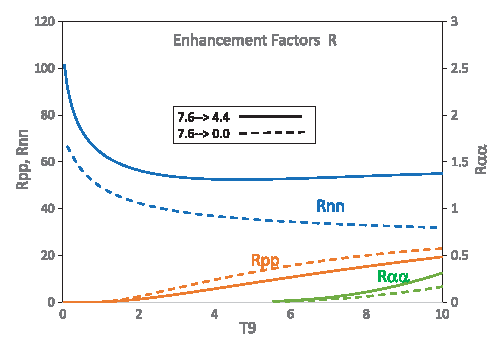
\includegraphics[clip, width=0.6\columnwidth]{R_T.eps}
  \caption[$\gamma$線による脱励起の寿命と粒子散乱による脱励起の寿命の比.]
          {$\gamma$線による脱励起の寿命と粒子散乱による脱励起の寿命の比~\cite{hotdensemedium}.
    Rnn,Rpp,R$\alpha\alpha$はそれぞれ中性子,陽子,$\alpha$粒子と散乱した際の寿命の比を表す.}
  \label{fig::R}
\end{figure}

$\rho\sim\SI{e6}{\gram\per\cubic\centi\metre}$のような高密度環境は宇宙の何処にあるだろうか.
一つの候補として超新星爆発が考えられる.
10--30 $\mathrm{M_{\odot}}$程度の大質量星は,重力崩壊を起こして星の一生を終える.
重力崩壊の際に恒星の中心にある鉄コアの温度が急激に上昇する.
極めて高い温度では高エネルギーの光子によって鉄コアの原子核が陽子や中性子に分解される.
また,密度が非常に高いため式\eqref{eq::neutronize}のように陽子が中性子へ変わる電子捕獲反応が起きる.
\begin{equation}
  {\rm p}+{\rm e}^{-} \rightarrow {\rm n}+\nu_{\rm e}
  \label{eq::neutronize}
\end{equation}
すると,恒星の中心に原始中性子星が形成される.
重力によって中心に降ってくる物質は原始中性子星によって跳ね返され,超新星爆発が起きる.
崩壊前の恒星が持っていた重力エネルギーが熱エネルギーに変換されるので,
原始中性子星の温度は\SI{e10}{\kelvin}に達する.
跳ね返った物質が膨張することで温度が下がっていき,
\SI{7e9}{\kelvin}ほどになると2つの陽子と2つの中性子が融合し$\alpha$粒子が合成される.
このとき,$\alpha$粒子と中性子が高密度かつ高温で存在する環境ができるのである.

\section{測定を行うべき中性子のエネルギー}
式\eqref{eq::R}から分かるように寿命の比$R$を計算するためには,
中性子と${}^{12}\mathrm{C}$の非弾性散乱断面積 [$\sigma_\mathrm{nn'} (E)$] のエネルギー分布が必要となる.
特に,式\eqref{eq::R}から分かるように$R$が$0_2^+$状態の励起エネルギーからのエネルギーに指数関数で依存しているので,
$0_2^+$状態へ励起させることができる中性子エネルギーの閾値付近における断面積が重要となる.
基底状態からの励起を考えると,重心系のエネルギーでは,$E=\SI{7.65}{\mega\electronvolt}$,
${}^{12}\mathrm{C}$の静止系における中性子のエネルギーでは$E_{\text{lab}} = \SI{8.35}{\mega\electronvolt}$である.
%特に,天体中で${}^{12}\mathrm{C}$と散乱した後に中性子が持つエネルギー領域を狙う必要がある.
%Beardら~\cite{hotdensemedium}が考えているような$T\sim\SI{e9}{\kelvin}$では,
%$k_{B}T\sim\SI{100}{\kilo\electronvolt}$である.% 1K = 8.61734e-5 eV
%このような中性子がHoyle状態 (Ex = \SI{7.65}{\mega\electronvolt}) の${}^{12}\mathrm{C}$と散乱すると,
%散乱後の中性子は$E_{\text{n}}\sim\SI{8}{\mega\electronvolt}$となる.
%つまり,式\eqref{eq::tau}に示した脱励起の寿命の計算には
%数 \si{\mega\electronvolt}のエネルギーを持つ中性子と${}^{12}\mathrm{C}$との断面積のエネルギー分布が必要となる.
図\ref{fig::crosssection_pres}~\cite{hotdensemedium}は${}^{12}\mathrm{C}$と中性子(上)または陽子(下)の
各実験室系エネルギーにおける非弾性散乱断面積のエネルギー分布を示す.
点で示される値は測定値,実線で示される値はTALYS による理論計算値を表す.
図\ref{fig::crosssection_pres} (上) から分かるように,
%数 \si{\mega\electronvolt}の領域におけるg.s. $\rightarrow$ Hoyle状態のデータがない.
$E_{\text{lab}} =$ \SIrange{8}{15}{\mega\electronvolt}の領域におけるg.s. $\rightarrow$ Hoyle状態の中性子の測定値がない.
そのため,このエネルギー領域での ${}^{12}\mathrm{C}(\mathrm{n},\mathrm{n}'){}^{12}\mathrm{C} (0_2^+)$ の
断面積の測定が必要となる.
\begin{figure}
  \centering
  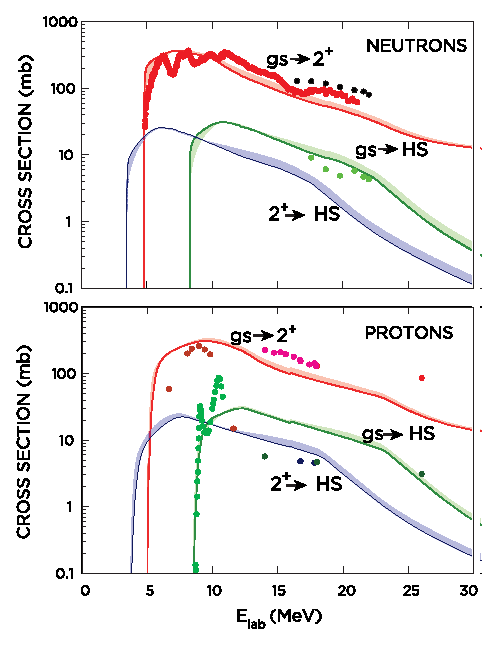
\includegraphics[clip,width=0.6\columnwidth]{cross_section_p_and_n.eps}
  \caption[${}^{12}\mathrm{C}$と中性子 (上段) および陽子 (下段) との非弾性散乱断面積.]
          {${}^{12}\mathrm{C}$と中性子 (上段) および陽子 (下段) との非弾性散乱断面積~\cite{hotdensemedium}.
  実線はTALYS~\cite{talys-1.0} を用いた理論計算,点は測定値を表す.}
  \label{fig::crosssection_pres}
\end{figure}

%本研究ではその第一歩として
%$E_{\text{n}} = \SI{14}{\mega\electronvolt}$の中性子を用いて断面積の測定を行い,
%${}^{12}\mathrm{C}(\mathrm{n},\mathrm{n}'){}^{12}\mathrm{C} (0_2^+)$反応の断面積測定の実現可能性を確認する.
%\SI{14}{\mega\electronvolt}は式\eqref{eq::dt}に示すデューテリウムとトリチウムの反応(DT 反応)を
%用いて生成可能なエネルギーである.
%この反応は2体反応であるため,放出角度により中性子のエネルギーが一意に決まる.%単色エネルギーの中性子となる.
%\begin{equation}
%  \mathrm{d} + \mathrm{t} \rightarrow \alpha\ (\SI{3.5}{\mega\electronvolt}) + \mathrm{n}\ (\SI{14}{\mega\electronvolt})
%  \label{eq::dt}
%\end{equation}
%単色エネルギーの中性子を用いることで,中性子のエネルギー測定を行う必要が無くなる.
%%核破砕で生成される
%%このDT 反応で生成される$14~{\rm MeV}$の中性子と炭素との反応は核融合炉の開発で重要である.
%ITER~\cite{iter}などの核融合炉ではこのDT 反応を用いて質量エネルギーを取り出す.
%核融合炉の中で生成される\SI{14}{\mega\electronvolt}の中性子は構造材の原子核と反応し損傷させるため,
%構造材の中に多く含まれる炭素との反応が詳しく調べられている~\cite{takahashietal,kondoetal}.
%${}^{12}\mathrm{C}(\mathrm{n},\mathrm{n}'+3\alpha)$反応の全断面積は\SI{209}{\milli\barn},
%分岐比は表\ref{tab::branchingratio}の通りである.
%また,微分断面積の角度分布を図\ref{fig::sig_angle_dist}に示す.
%これらの測定値と本研究での測定値を比較することによって測定方法の妥当性を確認することが可能となる.
%単色エネルギーの中性子を生成可能であること,他データと測定結果の比較が可能であることの2点より,
%測定方法の検証として\SI{14}{\mega\electronvolt}の中性子ビームを用いて
%${}^{12}\mathrm{C}(\mathrm{n},\mathrm{n}'){}^{12}\mathrm{C}(0_2^+)$反応の断面積の測定を行う.
%
%\begin{table}
%  \centering
%  \caption[${}^{12}\mathrm{C}(\mathrm{n},\mathrm{n}'+3\alpha)$反応のチャンネルとその分岐比.]
%          {${}^{12}\mathrm{C}(\mathrm{n},\mathrm{n}'+3\alpha)$反応のチャンネルとその分岐比~\cite{kondoetal}.
%            ${}^{12}\mathrm{C}$の励起状態から$3\alpha$に,${}^{9}\mathrm{Be}$の励起状態から$2\alpha$に崩壊する.}
%  \label{tab::branchingratio}
%  \begin{tabular}{lc}
%    \toprule
%    \multicolumn{1}{c}{Reaction channel} & Branching ratio (\%)\\
%    \midrule
%    ${}^{12}\mathrm{C}(\mathrm{n},\mathrm{n}'){}^{12}\mathrm{C}^{*}$(\SI{7.65}{\mega\electronvolt}) & 4\\
%    ${}^{12}\mathrm{C}(\mathrm{n},\mathrm{n}'){}^{12}\mathrm{C}^{*}$(\SI{9.64}{\mega\electronvolt}) & 33\\
%    ${}^{12}\mathrm{C}(\mathrm{n},\mathrm{n}'){}^{12}\mathrm{C}^{*}$(\SI{10.3}{\mega\electronvolt}) & 16\\
%    ${}^{12}\mathrm{C}(\mathrm{n},\mathrm{n}'){}^{12}\mathrm{C}^{*}$(\SI{10.84}{\mega\electronvolt}) & 6\\
%    ${}^{12}\mathrm{C}(\mathrm{n},\mathrm{n}'){}^{12}\mathrm{C}^{*}$(\SI{11.83}{\mega\electronvolt}) & 4\\
%    ${}^{12}\mathrm{C}(\mathrm{n},\alpha){}^{9}\mathrm{Be}^{*}$(\SIrange{1.68}{3.05}{\mega\electronvolt}) & 24\\
%    ${}^{12}\mathrm{C}(\mathrm{n},\alpha){}^{9}\mathrm{Be}^{*}$(\SI{4.7}{\mega\electronvolt}) & 13\\
%    \bottomrule
%  \end{tabular}
%\end{table}

\section{測定に用いる実験装置}
\label{seq::detector_using_experiment}
中性子によって励起された${}^{12}{\rm C} (0_2^+)$の崩壊によって放出された3つの$\alpha$粒子を測定することで,
断面積を決定する.
図\ref{fig::sig_angle_dist}は\SI{14}{\mega\electronvolt}の中性子と${}^{12}\mathrm{C}$との非弾性散乱の微分断面積である.
\SI{14}{\mega\electronvolt}の中性子と${}^{12}\mathrm{C}$の反応は
\ref{chap::experiment}章で説明する理由により既に測定されている.
入射中性子のエネルギーによらず図\ref{fig::sig_angle_dist}の微分断面積で散乱し,
励起した${}^{12}\mathrm{C}(0_2^+)$から$\alpha$粒子が等方的に崩壊すると仮定すると,
${}^{12}\mathrm{C} (0_2^+)$から放出された$\alpha$粒子は
図\ref{fig::alpha_E_En_dep_w_l}に示すエネルギーの分布を持つ.
横軸は入射中性子のエネルギー,縦軸は崩壊後の$\alpha$粒子のエネルギーである.
図\ref{fig::alpha_E_En_dep_w_l}から中性子のエネルギーに関わらず
$\alpha$粒子のエネルギーは約\SI{0.1}{\mega\electronvolt}が最頻値となっていることが分かる.
\SI{1}{\mega\electronvolt}より大きい領域は重心運動と同じ方向に放出された$\alpha$粒子が
ブーストされエネルギーが大きくなったものと考えられる.
一方,重心運動と異なる方向に放出された$\alpha$粒子は,
あまりブーストされずに典型的には励起エネルギーと3$\alpha$崩壊閾値の差分を3等分したエネルギー
($\SI{0.38}{\mega\electronvolt}\div 3 \sim \SI{0.1}{\mega\electronvolt}$) を持つ.
図\ref{fig::sig_angle_dist}から分かるように
${}^{12}\mathrm{C}(\mathrm{n},\mathrm{n}'){}^{12}\mathrm{C}(0_2^+)$反応では前方散乱の断面積が大きく,
${}^{12}\mathrm{C} (0_2^+)$が重心運動方向と異なる方向に散乱される確率が高い.
そのため,$\alpha$粒子はあまり重心運動によってブーストされる効果を受けずに,
中性子のエネルギーに関わらず\SI{0.1}{\mega\electronvolt}付近で最大となる.
中性子のエネルギーが\SI{14}{\mega\electronvolt}のときの分布を図\ref{fig::alpha_E_dist_high}に,
\SI{8.5}{\mega\electronvolt}のときの分布を図\ref{fig::alpha_E_dist_low}に示す.
図の塗りつぶし部分は最大値を中心に全体の8割となる領域を示している.
図\ref{fig::alpha_E_dist_high}では\SIrange{0}{600}{\kilo\electronvolt},
図\ref{fig::alpha_E_dist_low}では\SIrange{0.015}{505}{\kilo\electronvolt}である.
このような低エネルギーの$\alpha$粒子を効率よく検出するためには,
標的中で$\alpha$粒子が停止しないようにしなければならない.
例えば,\SI{500}{\kilo\electronvolt}の$\alpha$粒子ではおよそ\SI{350}{\micro\gram\per\square\centi\metre}の
炭素箔標的で停止してしまう.
更に低いエネルギーの$\alpha$粒子も検出しようとすると,更に標的を薄くしなければならない.
このような低エネルギー粒子の測定には,検出器そのものが標的となるアクティブ標的が有効である.
\begin{figure}
  \centering
  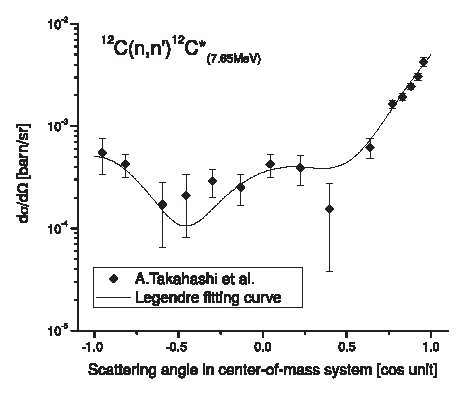
\includegraphics[clip, width=0.6\columnwidth]{cross_section_12C_n_n_12C_7.65.eps}
  \caption{\SI{14}{\mega\electronvolt}の中性子における
    ${}^{12}\mathrm{C}(\mathrm{n},\mathrm{n}'){}^{12}\mathrm{C} (0_2^+)$の微分断面積の角度分布~\cite{kondoetal}.}
  \label{fig::sig_angle_dist}
\end{figure}

図\ref{fig::alpha_theta_En_dep}は$\alpha$粒子の実験室系での角度分布である.
横軸は入射中性子のエネルギー,縦軸は$\alpha$粒子の入射中性子の運動方向に対する角度を表す.
$\alpha$粒子のエネルギー分布と同様に入射中性子のエネルギーにあまり依存していない.
入射中性子が\SI{14}{\mega\electronvolt}のときの角度分布を図\ref{fig::alpha_theta_dist_high}に,
\SI{8.5}{\mega\electronvolt}のときの角度分布を図\ref{fig::alpha_theta_dist_low}に示す.
図の塗りつぶしは最大値を中心に全体の8割となる領域を示している.
図\ref{fig::alpha_theta_dist_high}では\SIrange{7.5}{75.1}{\degree} である,
図\ref{fig::alpha_theat_dist_low}では\SIrange{5.5}{57.5}{\degree}である.
%この図からもわかるように広い角度領域に$\alpha$粒子は崩壊する.
このような広い角度に放出される3つの$\alpha$粒子すべてを効率的に検出するためには大立体角を覆う検出器が必要となる.

このような要求を満たす検出器として検出ガスを散乱標的として用いるtime projection chamber (TPC) が有効である.
TPC は荷電粒子のトラックを検出することができるガス検出器であり,
ALICE 実験~\cite{alice-tpc}やLEPS2~\cite{kobayakawa_thesis}などで広く用いられている.
アクティブ標的TPC を用いることで,低エネルギー荷電粒子を大立体角で検出することが可能となる.
近年,不安定核実験のためにMAYA~\cite{maya}やCAT~\cite{cat-tpc},AT-TPC~\cite{at-tpc}など
様々なアクティブ標的TPC が世界中で開発されている~\cite{active-tpc}.
その1つとして我々が開発したMAIKo ($\mu$-PIC based active target for inverse kinematics $_{\circ}$)
 TPC~\cite{maiko, mupic}がある.
近年,RCNP でMAIKo TPC を用いて低エネルギー$\alpha$粒子を測定する実験~\cite{Furuno2019}が行われた.
MAIKo TPC を用いることで低エネルギーの$\alpha$粒子を大立体角で検出することができる.
本研究ではMAIKo TPC を用いて${}^{12}\mathrm{C}(\mathrm{n},\mathrm{n}'){}^{12}\mathrm{C} (0_2^+)$反応を測定することを目指す.
\begin{figure}
  \centering
  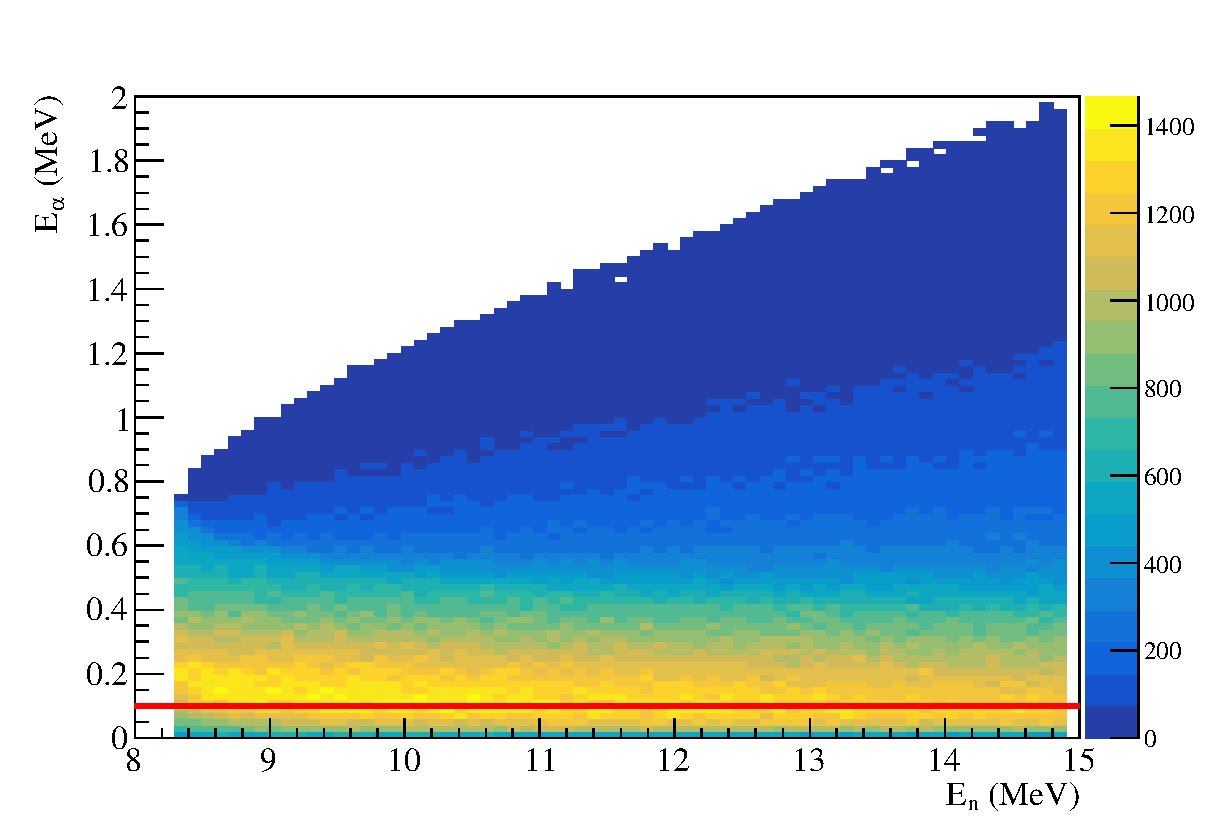
\includegraphics[clip, width=0.8\columnwidth]{alpha_E_En_dep_w_l.eps}
  \caption{${}^{12}\mathrm{C} (0_2^+)$から放出された$\alpha$粒子のエネルギー分布.
    横軸は入射中性子のエネルギー,縦軸は崩壊後の$\alpha$粒子のエネルギーである.
    赤い実線は$E_{\alpha}$ = \SI{0.1}{\mega\electronvolt}を表す.}
  \label{fig::alpha_E_En_dep_w_l}
\end{figure}
\begin{figure}
  \centering
  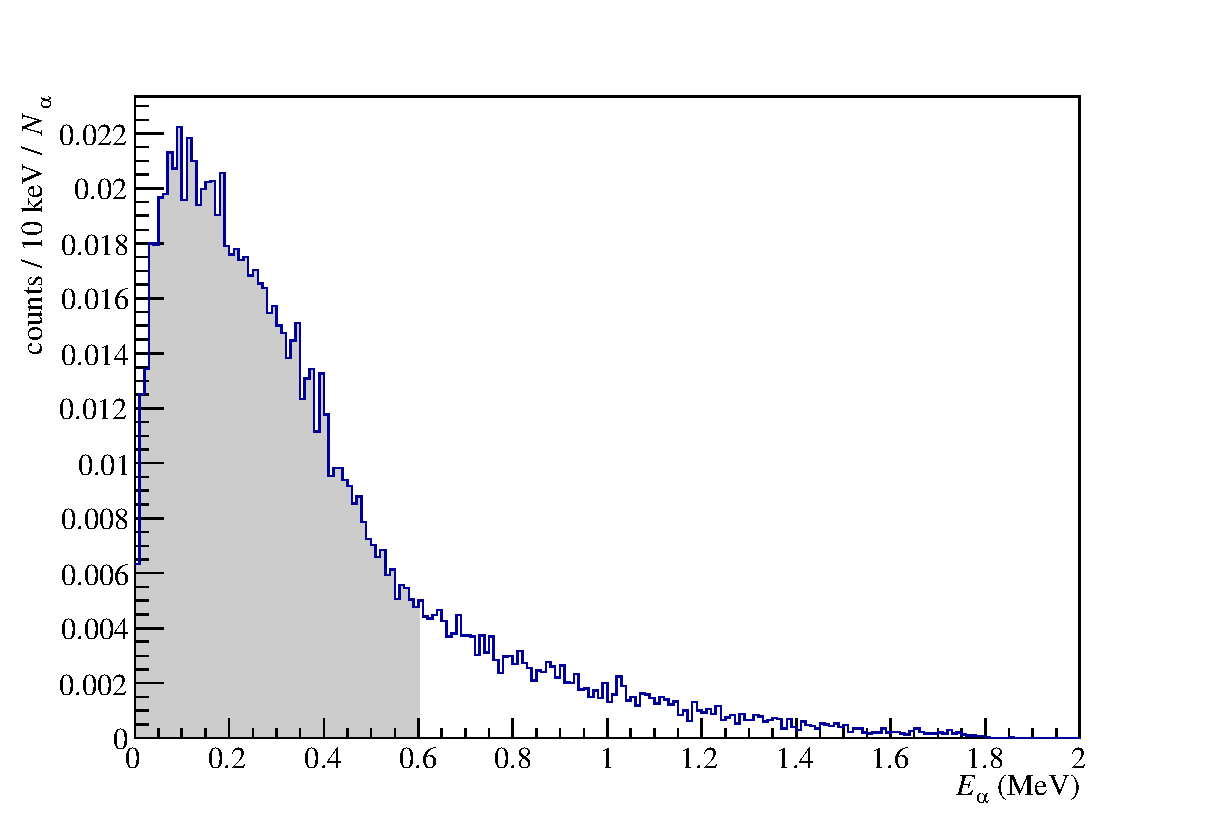
\includegraphics[clip, width=0.8\columnwidth]{alpha_E_dist_region_high.eps}
  \caption[${}^{12}{\rm C} (0_2^+)$から放出された$\alpha$粒子のエネルギー分布.]
          {$E_{\mathrm{n}}=\SI{14}{\mega\electronvolt}$のときの,
            ${}^{12}{\rm C} (0_2^+)$から放出された$\alpha$粒子のエネルギー分布.
            ${}^{12}\mathrm{C}$から放出される3つの$\alpha$粒子すべての分布を表している.}
          \label{fig::alpha_E_dist_high}
\end{figure}
\begin{figure}
  \centering
  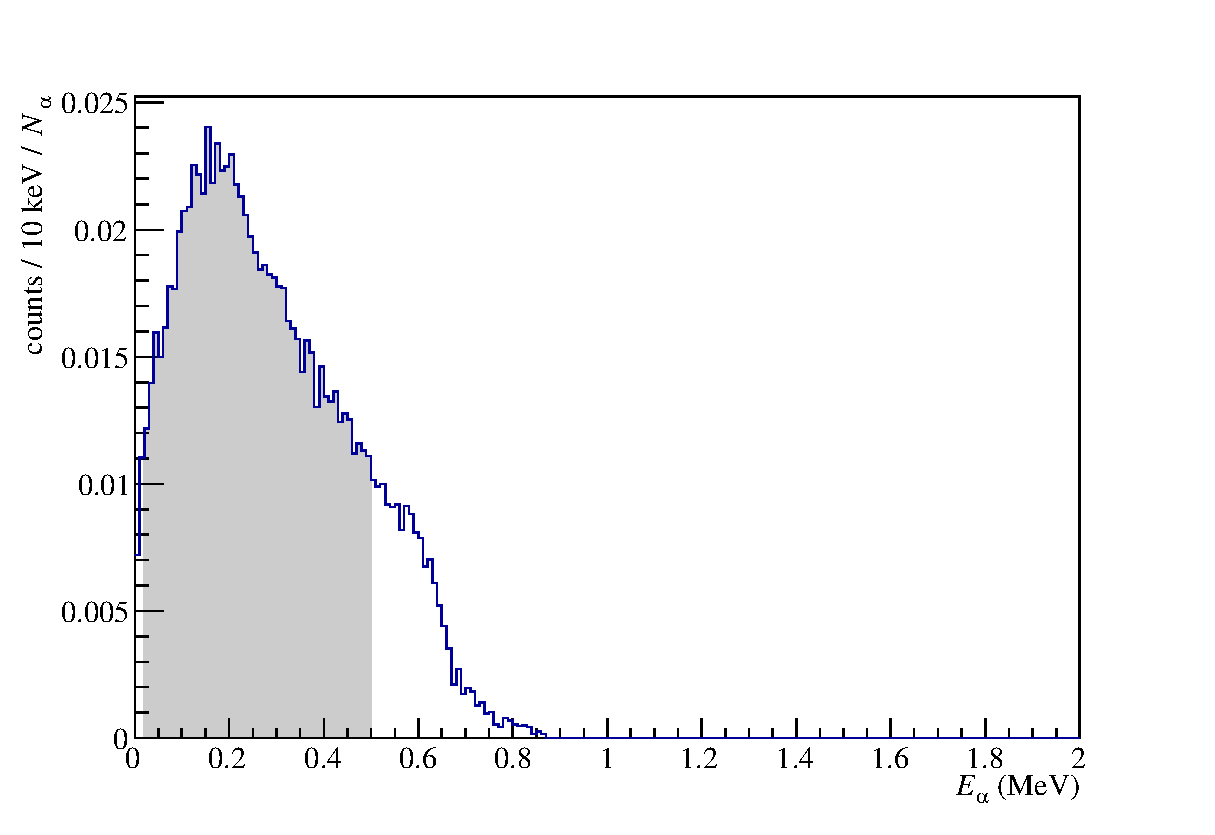
\includegraphics[clip, width=0.8\columnwidth]{alpha_E_dist_region_low.eps}
  \caption[${}^{12}{\rm C} (0_2^+)$から放出された$\alpha$粒子のエネルギー分布.]
          {$E_{\mathrm{n}}=\SI{8.5}{\mega\electronvolt}$のときの,
            ${}^{12}{\rm C} (0_2^+)$から放出された$\alpha$粒子のエネルギー分布.
            ${}^{12}\mathrm{C}$から放出される3つの$\alpha$粒子すべての分布を表している.}
          \label{fig::alpha_E_dist_low}
\end{figure}
\begin{figure}
  \centering
  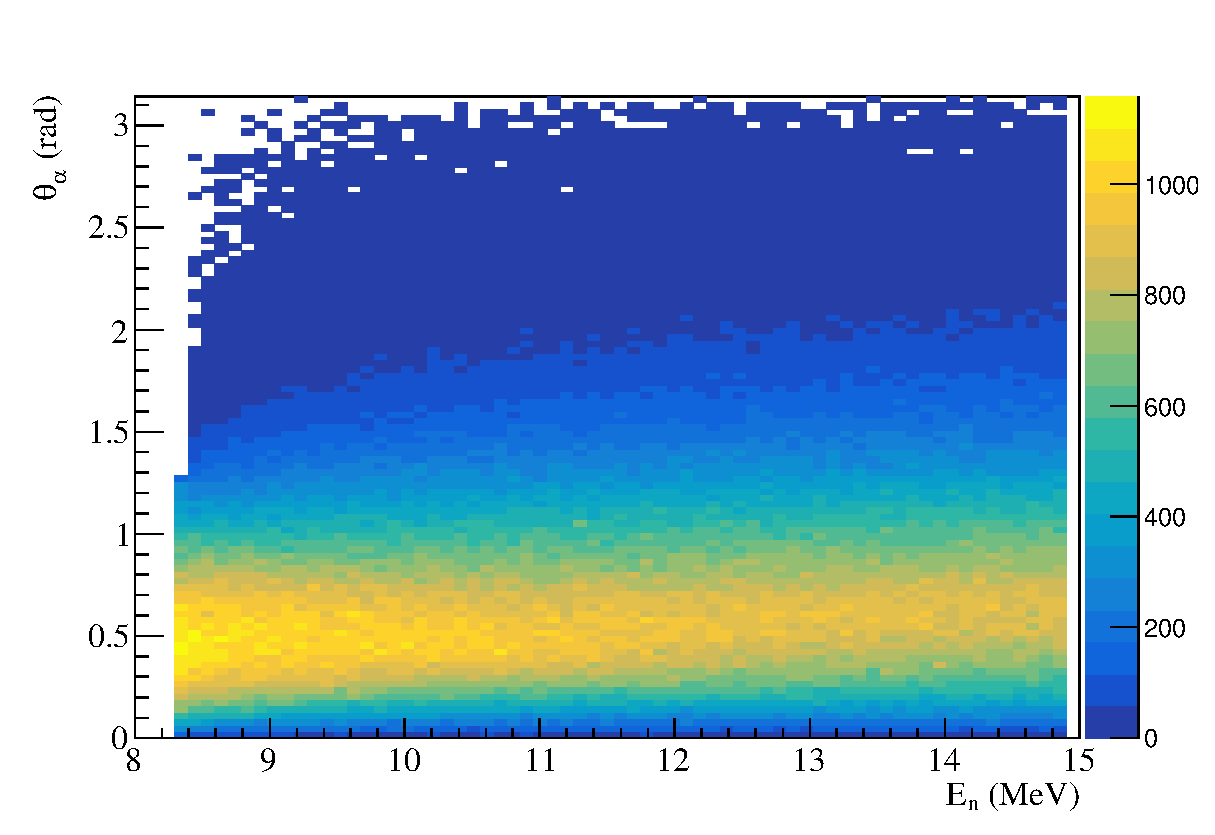
\includegraphics[clip, width=0.8\columnwidth]{alpha_theta_En_dep.eps}
  \caption{${}^{12}{\rm C} (0_2^+)$から放出された$\alpha$粒子の角度分布.}
  \label{fig::alpha_theta_En_dep}
\end{figure}
\begin{figure}
  \centering
  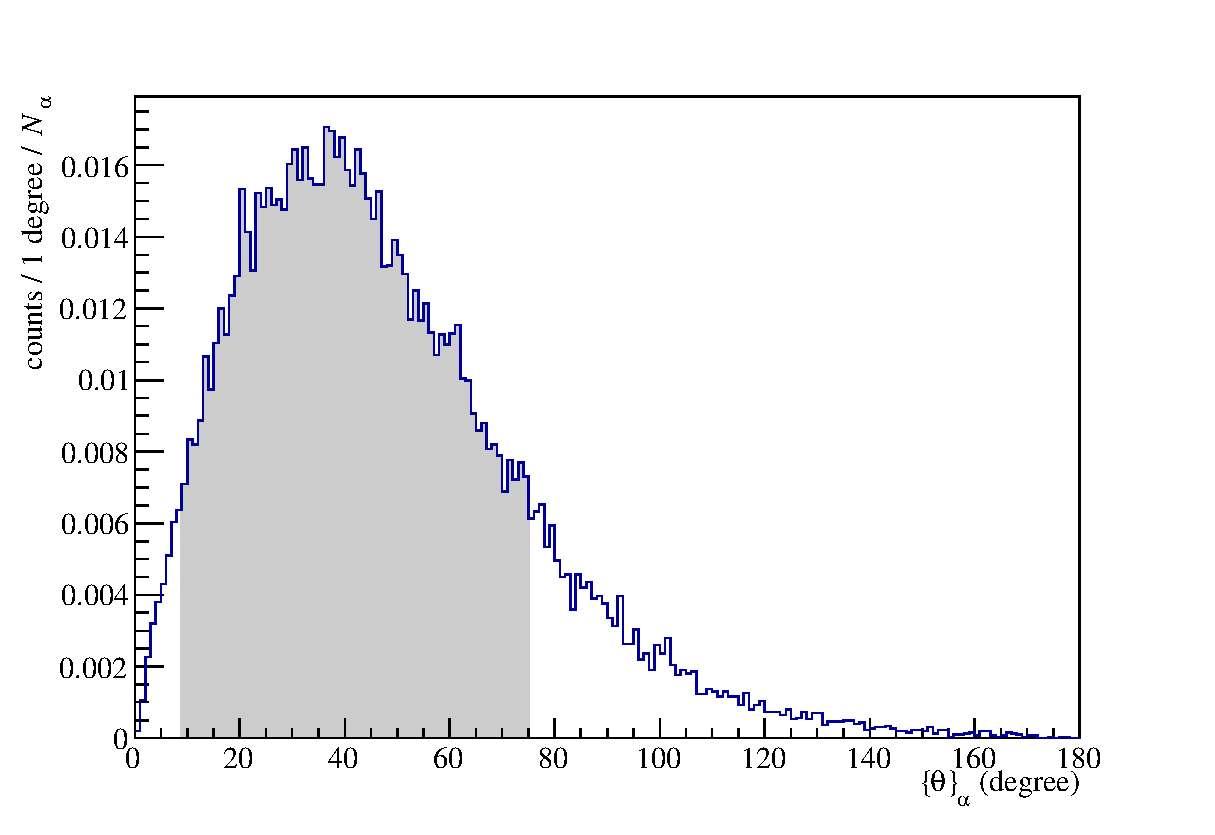
\includegraphics[clip, width=0.8\columnwidth]{alpha_theta_dist_region_high.eps}
  \caption[${}^{12}{\rm C} (0_2^+)$から放出された$\alpha$粒子の角度分布.]
          {$E_{\mathrm{n}}=\SI{14}{\mega\electronvolt}$のときの,
            ${}^{12}{\rm C} (0_2^+)$から放出された$\alpha$粒子の角度分布.
            ${}^{12}\mathrm{C}$から放出される3つの$\alpha$粒子すべての分布を表している.
          }
  \label{fig::alpha_theta_dist_high}
\end{figure}
\begin{figure}
  \centering
  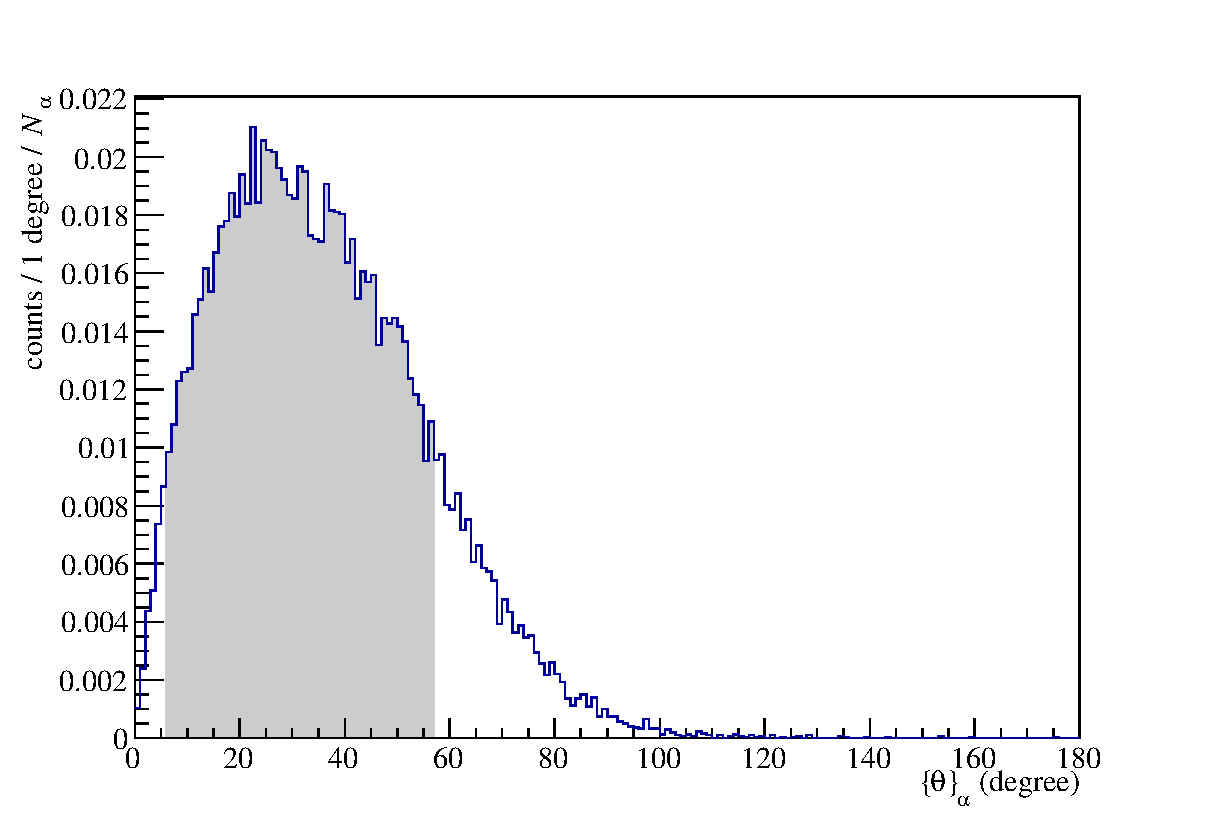
\includegraphics[clip, width=0.8\columnwidth]{alpha_theta_dist_region_low.eps}
  \caption[${}^{12}{\rm C} (0_2^+)l$から放出された$\alpha$粒子の角度分布.]
          {$E_{\mathrm{n}}=\SI{8.5}{\mega\electronvolt}$のときの,
            ${}^{12}{\rm C} (0_2^+)$から放出された$\alpha$粒子の角度分布.
            ${}^{12}\mathrm{C}$から放出される3つの$\alpha$粒子すべての分布を表している.
          }
  \label{fig::alpha_theta_dist_high}
\end{figure}
%ピーク周りに8割を取ってくると0.13 rad -- 1.31 rad, 0 -- 0.595 MeV

%また,TPC は荷電粒子のトラックを検出することができる検出器である.
%荷電粒子を入射粒子として用いる実験では,標的粒子と散乱しなかった入射粒子のトラックも検出する.
%このような事象は背景事象となる.
%本研究では中性子を入射するため,そのような背景事象は発生しない.
%そのため,高強度の中性子ビームを用いた実験が可能であり,
%散乱事象を効率的に検出することができる.

\section{本研究の目的}
${}^{12}\mathrm{C}(\mathrm{n},\mathrm{n}'){}^{12}\mathrm{C} (0_2^+)$反応の断面積測定は,
低エネルギーの$\alpha$粒子を検出する必要がある.
\ref{seq::detector_using_experiment}節で述べたように,
MAIKo TPC を用いれば効率的に3つの低エネルギー$\alpha$粒子を検出することが可能となる.
しかし,崩壊してできた$\alpha$粒子が持つ運動エネルギーは広がりを持ち,数十倍違うこともある.
そのため,より効率的に全ての粒子を測定するための条件を検討する必要がある.
MAIKo TPC では使用する検出ガスの種類,圧力,電圧等の多くのパラメータを調整することができる.
本研究では効率的に$\alpha$粒子を検出することができる検出ガスの候補を複数選出し,
$\alpha$線源を用いて性能試験を行う.
それらのガスについて中性子との散乱で${}^{12}\mathrm{C}$原子核が3つの$\alpha$粒子に崩壊するイベントをシミュレートし,
MAIKo TPC から得られるであろう画像を生成する.
シミュレーションで生成した画像に対して解析を行い,検出効率,エネルギー分解能,角度分解能を評価する.
評価結果から実験で用いる検出ガスを決定する.
また,正しく解析を行える割合やこの測定方法で期待される収量の評価を行い,実験の実現可能性を検討する.
\end{document}
